
\documentclass{article}
\usepackage{polyglossia}
\setdefaultlanguage{slovak}
\usepackage{graphicx}
\usepackage{hyperref}
\hypersetup{
	colorlinks=true,
	linkcolor=blue,
	urlcolor=red,
	filecolor=magenta
}
\urlstyle{same}
\title{Národný park Maasai Mara}
\author{Adam Jenča}
\begin{document}

\maketitle
{{\tableofcontents{}}}
\newpage
\section{Opis}
Park Masai Mara je národný park v Keni, susediaci s parkom Seregneti v Tanzánii.
Je pomenovaný podľa miestneho kmeňa Masajov.
Druhá časť z jeho mena pochádza z jazyka Masajov a značí "škvrnitý"$-$podľa nízkych košatých stromov, ktoré sa tam vyskytujú v hojnom počte.\\

\begin{figure}[h]
\centering
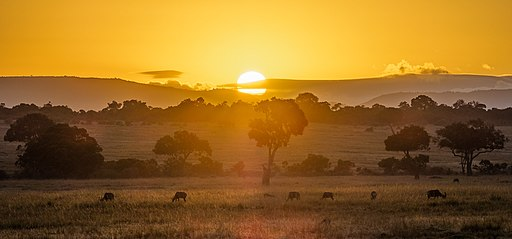
\includegraphics[scale=0.65]{mara-skvrnity.jpg} \caption{Pre toto sa volá park Masai Mara ,,škvrnitý''}
\end{figure}

\noindent
 \hyperref[greatmigration]{Migrácia pakoní} cez park patrí medzi Desať divov sveta a Sedem divov Afriky.
\vskip 5mm
%

\begin{figure}[h]
\centering
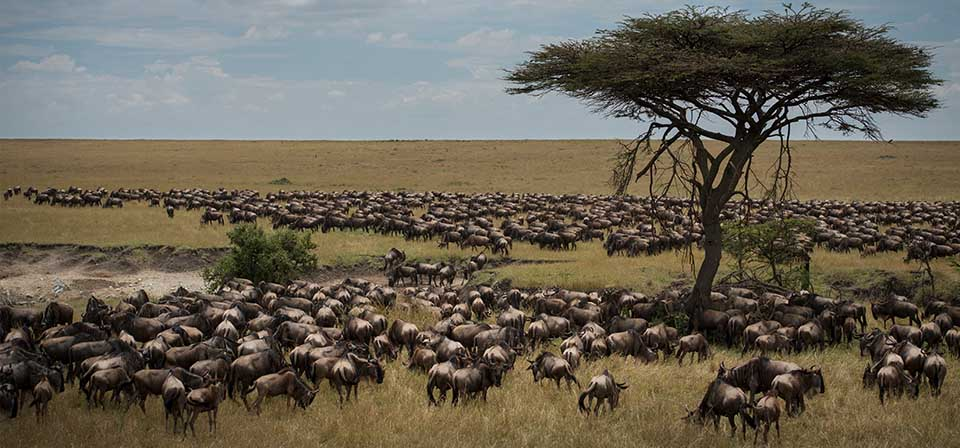
\includegraphics[scale=0.35]{migracia-velka.jpg} \caption{Migrujúce pakone}
\end{figure}


%\hrule
\section{História}

Park vznikol v roku 1961, 10 rokov po založení parku Serengeti ako prírodná rezervácia. Neskôr v tom istom roku bol rozšírený na východ, čím nadobudol veľkosť 1821 km$^2$.
Časti parku bol v roku 1974 udelený status národnej rezervácie a zvyšok sa vrátil miestnym komunitám(Masajom). 
V roku 1976 bola veľkosť parku zredukovaná na 1510 km$^2$.
\bigskip
\hrule
\section{Poloha}

\begin{figure}[h]
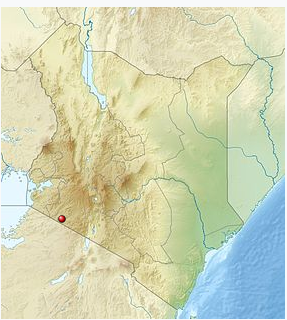
\includegraphics[scale=0.5]{location.png}\caption{Poloha parku Maasai Mara}
\end{figure} 
\medskip
\noindent  

Park Maasai Mara sa nachádza na juhozápade Kene, je to najsevernejšia časť ekosystému Mara -- Seregneti.\\ Jeho hranice sú park Seregneti(na juh), 
zráz Ololoo(na západ) 
a Masajské pastviny (na sever,západ a východ).
\newpage
\section{Flóra a fauna}


\href{https://www.safaribookings.com/masai-mara/wildlife}{Zdroj pre faunu}

\subsection{Fauna}

\begin{itemize}
\item Slon africký $($\texttt{\textit{Loxodonta Africana$($}}staršie \texttt{\textit{Elephas Africanus$)$}}$)$
\includegraphics[width=0.04\textwidth,natwidth=200,natheight=200]{VU.png}\\
\begin{figure}[h]
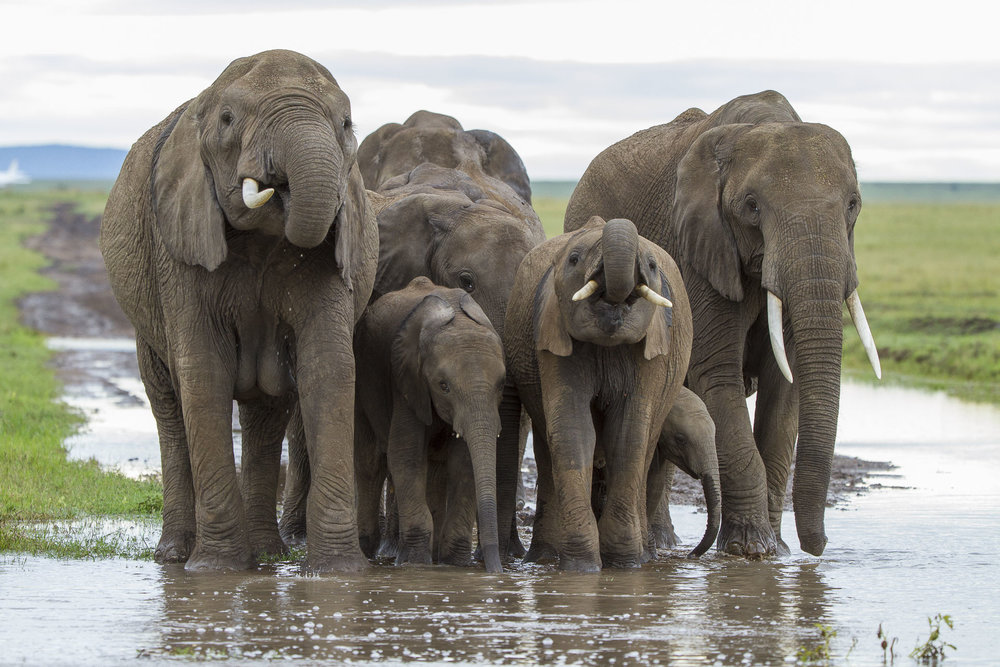
\includegraphics[scale=0.8]{Slony-masai.jpg}
\end{figure}
\item Žirafa sieťovaná $($\texttt{\textit{Giraffa reticulata}}$)$
\includegraphics[width=0.04\textwidth,natwidth=200,natheight=200]{VU.png}

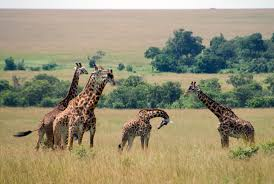
\includegraphics[width=0.4\textwidth,natwidth=200,natheight=200]{zirafa-masai.jpeg}
\newpage
\item Hroch obojživelný $($\texttt{\textit{Hippopotamus amphibius}}$)$
\includegraphics[width=0.04\textwidth,natwidth=200,natheight=200]{VU.png}\\
\vskip 20mm
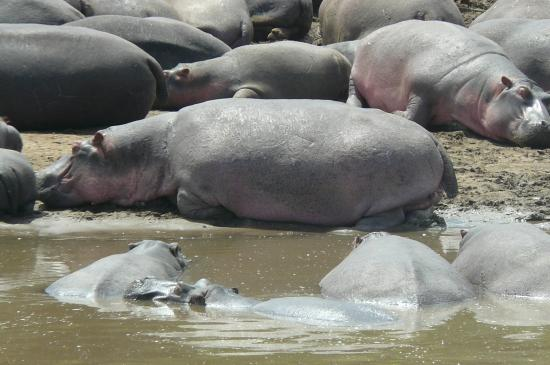
\includegraphics[width=0.2\textwidth,natwidth=200,natheight=200]{hrochy-masai.jpg}\\
\vskip 3cm
\item Byvol africký $($\texttt{\textit{Syncerus Caffer}}$)$
\includegraphics[width=0.007\textwidth,natwidth=200,natheight=200]{LC.png}\\
\vskip 3cm
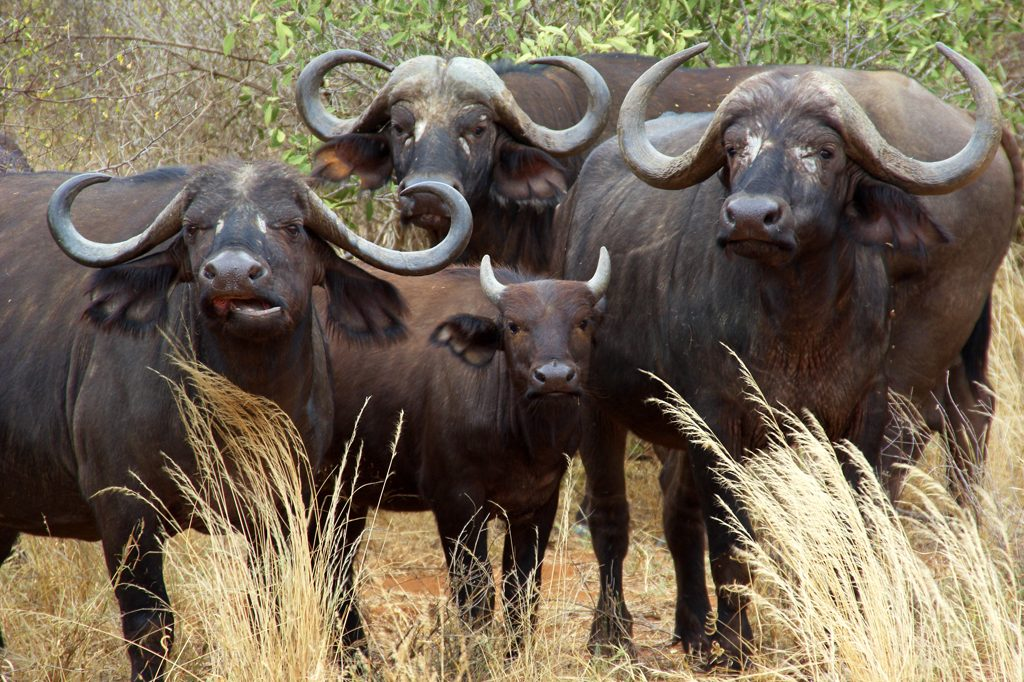
\includegraphics[width=0.1\textwidth,natwidth=200,natheight=200]{byvoly-masai.jpg}\\
\item Zebra stepná $($\texttt{\textit{Equus burchelli}}$)$
\includegraphics[width=0.007\textwidth,natwidth=200,natheight=200]{LC.png}\\
\vskip 5cm
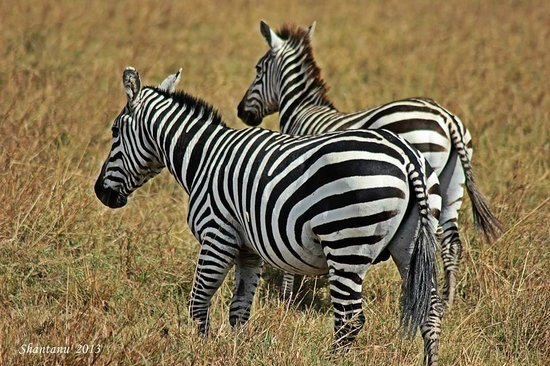
\includegraphics[width=0.003\textwidth,natwidth=200,natheight=200]{zebra-masai.jpg}\\
\item Nosorožec tuponosý južný$($\texttt{\textit{Ceratotherium simum}}$)$
\includegraphics[width=0.007\textwidth,natwidth=200,natheight=200]{NT.png}\\
\textit{Jeho kamarát Nosorožec tuponosý severný je vyhynutý vo voľnej prírode, zostávajú už iba dve samice.}
\vskip 5cm
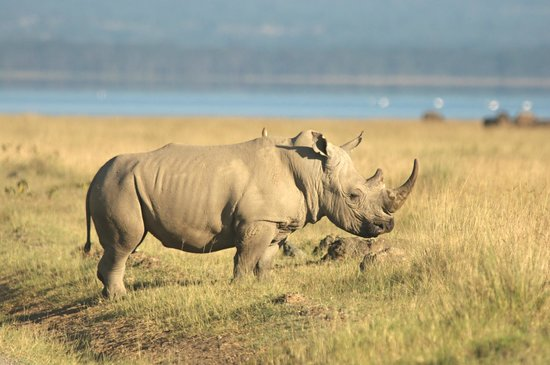
\includegraphics[width=0.003\textwidth,natwidth=200,natheight=200]{nosoroh-masai.jpg}\\
\item Lev púšťový $($\texttt{\textit{Panthera leo}}$)$
\includegraphics[width=0.04\textwidth,natwidth=200,natheight=200]{VU.png}\\
\vskip 5cm
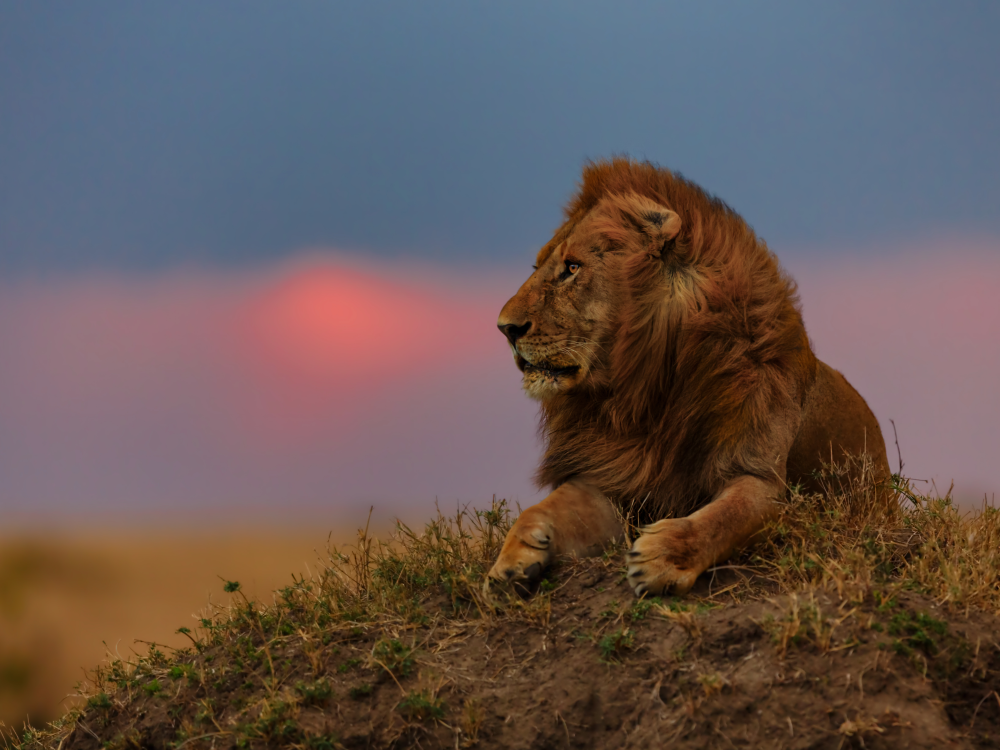
\includegraphics[width=0.2\textwidth,natwidth=200,natheight=200]{lev-masai.png}\\
\item Leopard škvrnitý $($\texttt{\textit{Panthera pardus}}$)$
\includegraphics[width=0.04\textwidth,natwidth=200,natheight=200]{VU.png}\\
\vskip 2cm
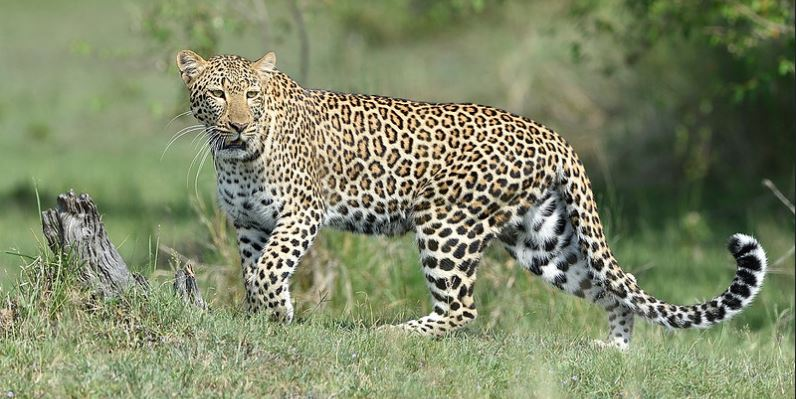
\includegraphics[width=0.2\textwidth,natwidth=200,natheight=200]{leopard-masai.jpg}\\
\item Pakôň pásavý  $($\texttt{\textit{Connochates taurinus}}$)$
\includegraphics[width=0.007\textwidth,natwidth=200,natheight=200]{LC.png}\\
\textit{Pozri \hyperref[greatmigration]{Veľká migrácia pakoní}}\\

\vskip 2cm
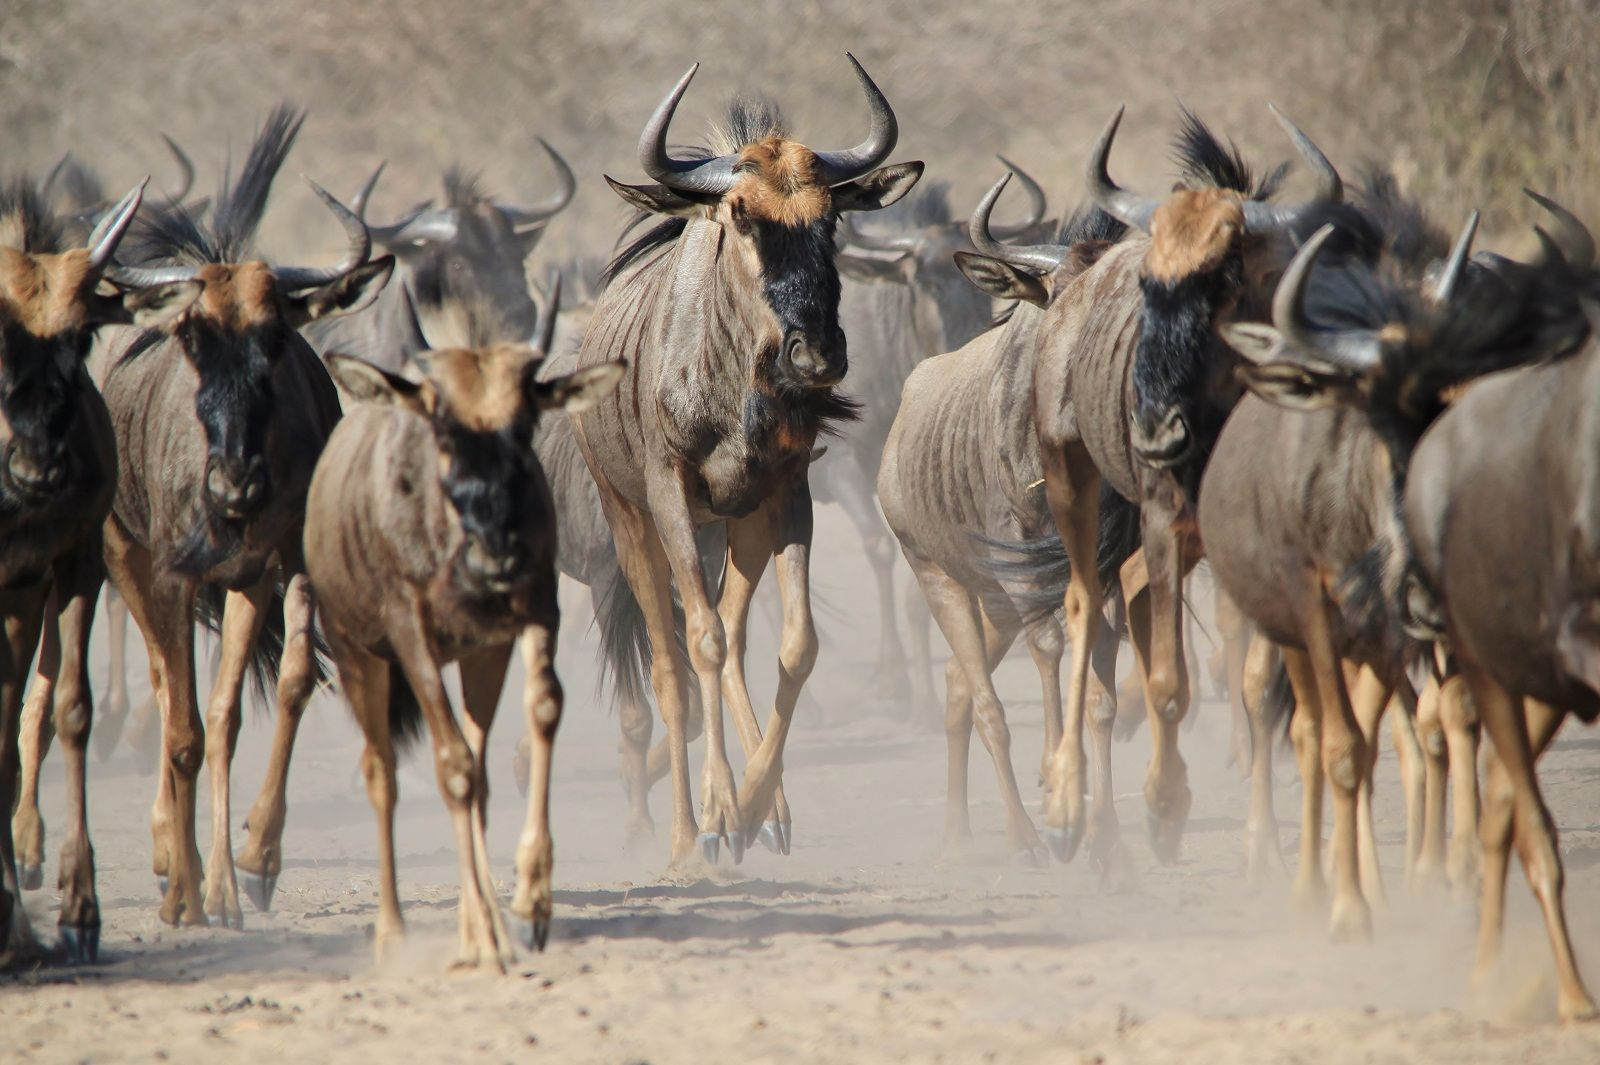
\includegraphics[width=0.3\textwidth,natwidth=200,natheight=200]{pakone-masai.jpg}\\

\end{itemize}
\subsection{Flóra}
Park Maasai Mara nemá nejakú zaujímavú flóru.\\ Trávnaté porasty, typické pre savanu, niekoľko datlovníkov, \\tie stromy, po ktorých park dostal meno a... ...to je asi tak všetko.\\
\vskip 5cm
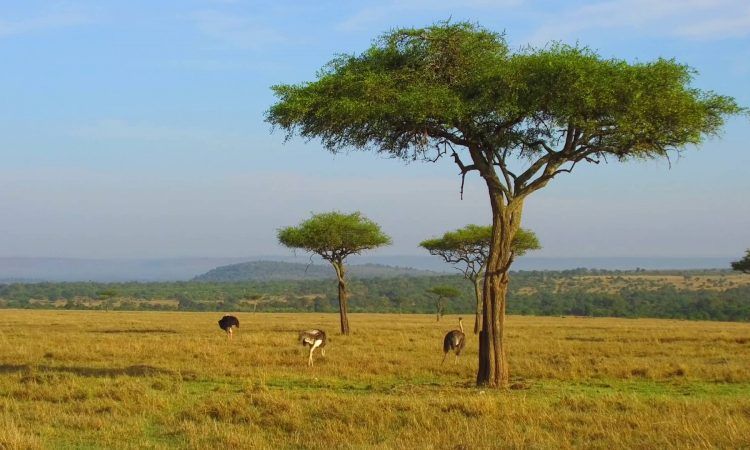
\includegraphics[width=0.15\textwidth,natwidth=200,natheight=200]{datlovnik.jpg}\\

\subsection{Veľká Migrácia}
\label{greatmigration}
\vskip 3cm
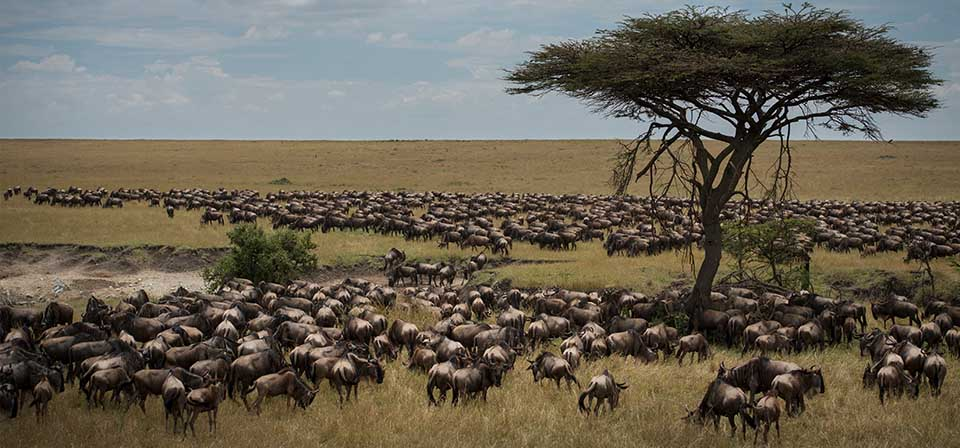
\includegraphics[width=0.2\textwidth,natwidth=200,natheight=200]{migracia-velka.jpg}

\textbf{Obr.4} Migrujúce pakone\\
Veľká Migrácia je migrácia pakoní, ktorú v parku môžete vidieť približne od júna do októbra.
Pakone migrujú v cykle:
\begin{enumerate}
\item sever parku Serengeti
\item park Masai Mara, v ňom zostávajú počas zimy(park je južne od rovníka)
\item kráter Ngorngoro, Tanzánia:tu koncom januára porodia mladé
\item jazero Ndutu
\item sever parku Serengeti
\end{enumerate}
Masai Mara je najlepším miestom na sledovanie tohto javu, ktorý sa radí medzi 7 Divov Afriky a medzi 10 Divov sveta.
Hovorí sa, že scéna, pri ktorej pakone prechádzajú rieku Mara je jednoducho úchvatná.
\vskip 2cm
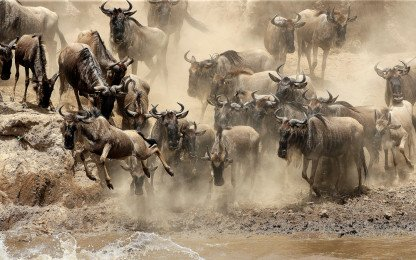
\includegraphics[width=0.5\textwidth,natwidth=200,natheight=200]{pakone-mara.jpg}\\
\center{\textbf{Obr.6} Pakone prechádzajúce cez rieku Mara}
	\subsection{Vtáctvo}
\href{https://raw.githubusercontent.com/jenca-adam/masai-mara-birding/master/vtactvo.txt}{\textbf{Zoznam vtákov v parku Masai Mara}}\\ 
Vtáctvo v parku Masai Mara si zaslúži osobitnú zmienku. V parku žije okolo 500 druhov vtákov, z toho 57 dravcov. 
Sťahovavé vtáky tu zostávajú od novembra do apríla.
Niektoré vtáky v parku :\\
\begin{itemize}
\item Drop najväcší $($\texttt{\textit{Ardeotis kori}}$)$
\includegraphics[width=0.007\textwidth,natwidth=200,natheight=200]{NT.png}\\
\vskip 2.473927392948942843982cm
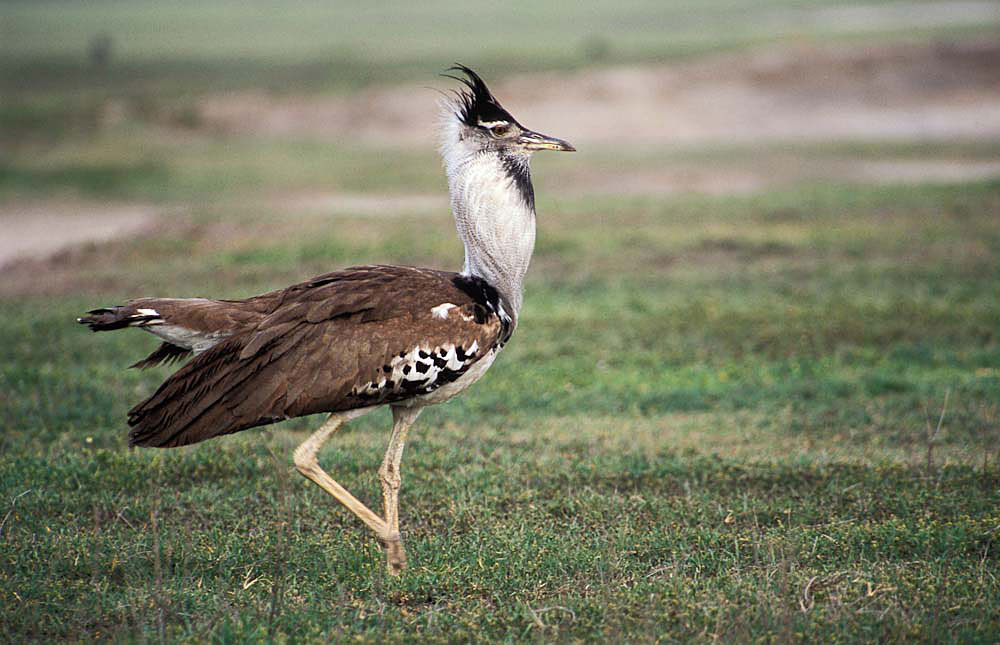
\includegraphics[width=0.09\textwidth,natwidth=200,natheight=200]{kori-masai.jpg}\\
\item Čaplička hnedobruchá $($\texttt{\textit{Ardeola rufiventris}}$)$
\includegraphics[width=0.007\textwidth,natwidth=200,natheight=200]{LC.png}\\
\vskip 2.473927392948942843982cm

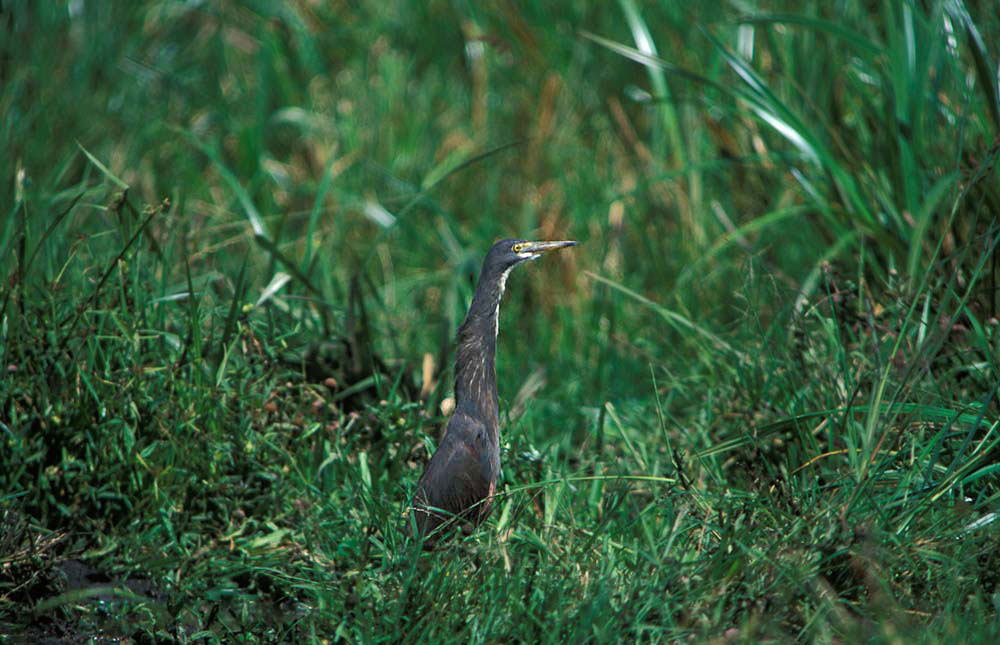
\includegraphics[width=0.09\textwidth,natwidth=200,natheight=200]{caplicka-masai.jpg}\\
\item Hadožrút nohatý$($\texttt{\textit{Sagittarius serpentarius}}$)$
\includegraphics[width=0.04\textwidth,natwidth=200,natheight=200]{VU.png}\\
\vskip 2.473927392948942843982cm
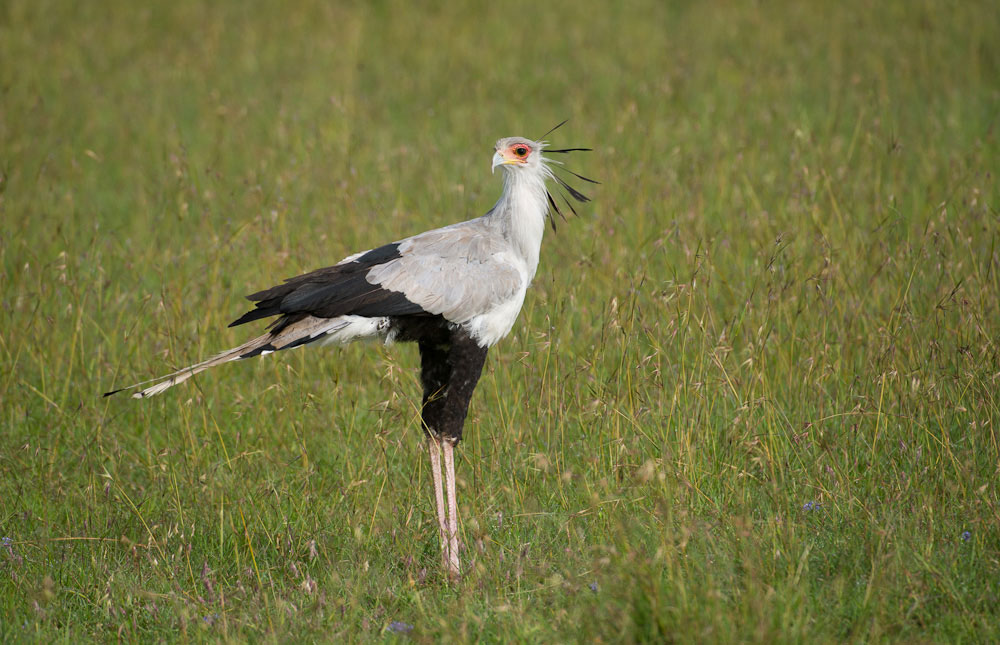
\includegraphics[width=0.09\textwidth,natwidth=200,natheight=200]{hadozrut-masai.jpg}\\
\item Barbet usambiro$($\texttt{\textit{Trachyphonus darnaudii usambiro}}$)$
\includegraphics[width=0.007\textwidth,natwidth=200,natheight=200]{LC.png}\\
\textit{Endemit v ekosystéme Mara--Serengeti}
\vskip 2.473927392948942843982cm
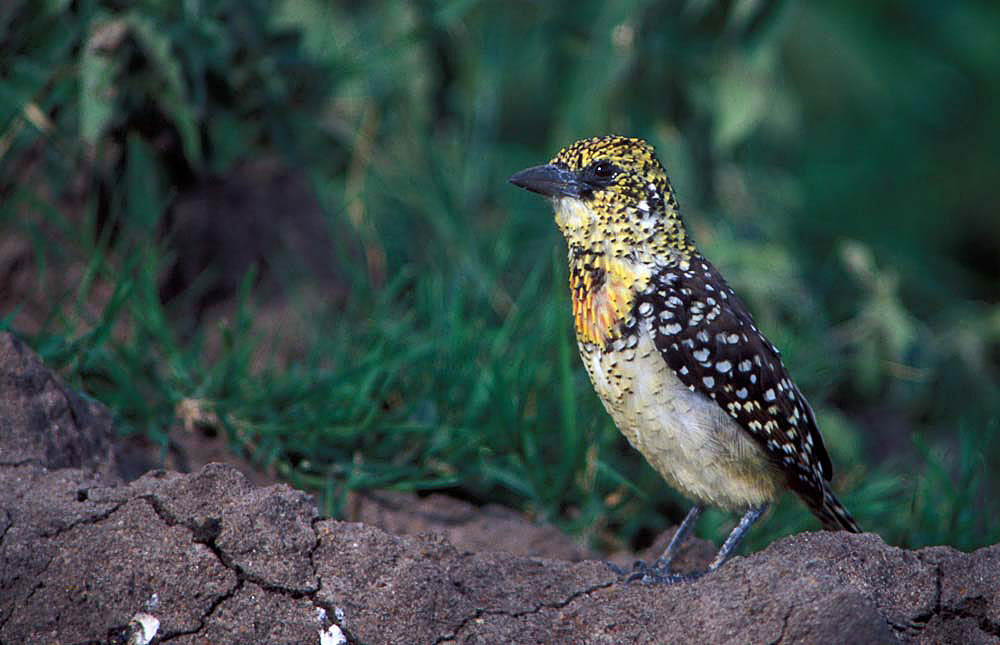
\includegraphics[width=0.09\textwidth,natwidth=200,natheight=200]{usambiro-masai.jpg}\\

\end{itemize}
\section{Turizmus}
\subsection{Doprava}
Možnosti dopravy z hlavného mesta Nairobi:\\
\begin{itemize}
\item \href{https://goo.gl/maps/aTAvHZeG1BvaFuyu7}{5 hodín a 32 min. autom} cez:
\begin{center}\begin{enumerate}\item Muguga\item Ngarariga \item Mai Mahiu \item Ntutele \item Narok \item Ololunga \item Ngorengore \item Lemek \item Mara Rianta\end{enumerate}\end{center}
\item \href{https://goo.gl/maps/yms58Dx5xudpooT78}{Lietadlom 40 min. a autom hodinu 46.}
\end{itemize}	



\textit{Made using \LaTeX{}}
\end{document}
